\documentclass{article}

\usepackage[utf8]{inputenc}
\usepackage[T1]{fontenc}
\usepackage[norsk,english]{babel}   %norsk først så engelsk, så engelsk blir prioritert
\usepackage{graphicx}
\usepackage{amsmath}
\usepackage{listings}
\usepackage{multicol}
\usepackage[margin=2.54cm]{geometry}
\usepackage{wrapfig}

%Definerer hyperlinker og dens farger
\usepackage{hyperref}
\hypersetup{
    colorlinks,
    citecolor=black,
    filecolor=black,
    linkcolor=blue,
    urlcolor=blue
}

%-----------------------------------

%Definerer farger til kodeeksemplene i PDF-en
\usepackage{color}

\definecolor{codegreen}{rgb}{0,0.6,0}
\definecolor{codegray}{rgb}{0.5,0.5,0.5}
\definecolor{codepurple}{rgb}{0.58,0,0.82}
\definecolor{backcolour}{rgb}{0.95,0.95,0.92}

\lstdefinestyle{mystyle}{
    backgroundcolor=\color{backcolour},
    commentstyle=\color{codegreen},
    keywordstyle=\color{magenta},
    numberstyle=\tiny\color{codegray},
    stringstyle=\color{codepurple},
    basicstyle=\footnotesize,
    breakatwhitespace=false,
    breaklines=true,
    captionpos=b,
    keepspaces=true,
    numbers=left,
    numbersep=5pt,
    showspaces=false,
    showstringspaces=false,
    showtabs=false,
    tabsize=2
}

\lstset{style=mystyle}

%------------------------------------

\setlength{\parindent}{0pt}
\setlength{\columnsep}{5mm} %column separation
\setlength{\columnsep}{10mm}

\setlength{\tabcolsep}{18pt}
\renewcommand{\arraystretch}{1.5}

\iffalse
If you want to change this temporarily, you can write:
\savegeometry{mydefaultgeometry}
\newgeometry{margin=3in}
And then later you can call:
\loadgeometry{mydefaultgeometry}
\fi

\begin{document}

\addtocounter{page}{0}

\title{Project 2 \\
      \large For the course FYS3150}
\date{\today \\
    \vspace{1mm}
    \large Week 37 - 40}

\author{Erik Grammeltvedt, Erlend Tiberg North and Alexandra Jahr Kolstad}

\maketitle

%\newpage

%------------Her starter skrivingen-----------------------------------------
\vspace{1cm}

\tableofcontents

\vspace{1cm}

%---------------------------------------
%\begin{multicols}{2}

\newpage
\clearpage


Abstract: short motivation and presentation of the results and the findings \\

Introduction: you want to motive the reader about the problem and why you want solve it \\

Theory: explaining the theory behind the solution method and the problem \\

method/implementation: how you implement the solution in order to fix/solve the problem \\

results/graphs/tables: presenting the results \\

discussion: Discussing the result from previous section \\

conclusion: concluding the findings, your neutral opinion, etc… and future work \\

appendix:How you derived your method, theory, etc… \\

\begin{itemize}

  \item How many similarity transformations are needed before you reach a result
  where all non-diagonal matrix elements are essentially zero?  \textit{Besvart i discussion}

  \item Try to estimate the number of transformations and extract a behavior as function of the dimension- ality of the matrix. \textit{Besvart i discussion}

  \item Compare your results with the analytical ones. \textit{Besvart i discussion og noe i results}

  \item Comment your results (here you could for example compute the time needed for both algorithms for a given dimensionality of the matrix). \textit{Besvart i discussion og noe i results}

  \item Try to figure out other tests your code should pass, based either on the mathematical properties of the algorithms or more program specific tests. Implement at least two unit tests in this project. \textit{Besvart i koden, men tenker å kommentere hvorfor valgte disse i method}

  \item Study the results as functions of the number of integration points N and your approximation to $\rho$ max. The analytical results with our scaling for the one-electron energies are $\lambda$ = 3, 7, 11, 15, . . . .

  \item How many integration points do you need in order to reproduce the analytical results with say four leading digits after the decimal point?

  \item Comment the results for the lowest state (ground state) as function of varying strengths of $ \omega$ r.

\end{itemize}



%----------Abstract-------------------------------
\vspace{1cm}

\section{Abstract} \label{sec:Abstract}

bla bla bla bla bla bla bla




%--------------Introduction------------------------------
\vspace{1cm}

\section{Introduction} \label{sec:Introduction}

All programs are found at our \href{https://github.com/Erikbgram/Fys3150}{GitHub-repository}. \\

\textbf{Hvilke filer som er til hvilke oppgaver} \\

Our project consists of the files \texttt{jacobimethod.cpp} and \texttt{plot\_data.py}. For exercises \textbf{b)} through \textbf{e)} we use the file \texttt{jacobimethod.cpp}. Also for exercise \textbf{b)} we have the file \texttt{plot\_data.py}.

This article is seperated into sections with some subsections.

%--------------- Theory ------------------------------------
\vspace{1cm}

\section{Theory} \label{sec:Theory}

\subsection{Orthogonality of a unitary transformation} \label{sec:orthogonality}

Firstly (?) we are going to prove that $\vec{w}_i = U \vec{v}_i$ is an orthogonal or unitary transformation that preserves the dot product and orthogonality. We start by multiplying $\vec{w}_j ^T$ with $\vec{w}_i$ to take the vector product, also called the dot product. If the vector product of these vectors is equal to $\delta_{ij}$, given by $\vec{v}_j ^T \vec{v}_i = \delta_{ij}$ in the exercise, then the dot product and orthogonality is preserved. In this exercise we assume that $U^T U = I$, where $I$ is the identity matrix, because this defines a unitary matrix $U$ which we compute with in this exercise. \\

The vector product is calculated as followed:

\begin{align*}
  \vec{w}_j ^T \vec{w}_i &= (U \vec{v})^T U \vec{v}_i \\
  &= \vec{v}_j ^T U^T U \vec{v}_i \\
  &= \vec{v}_j ^T \vec{v}_i \\
  &= \delta _{ij}
\end{align*}

The vector product of $\vec{w}_j ^T$ and $\vec{w}_i$ is $\delta_{ij}$, which proves that the dot product and orthogonality is preserved for the transformation.

In this prject we compute with a symmetric matrix, similar to the matrix \textbf{A} in project 1. This matrix is given by the matrix equation

  \begin{equation*} \label{eq:fullmatrixeq}
    \begin{bmatrix}
        d & a & 0 & \dots & 0 & 0 \\
        a & d & a & \dots & 0 & 0 \\
        0 & a & d & \dots & 0 & 0 \\
        \vdots & \vdots & \vdots & \ddots & \vdots & \vdots \\
        0 & 0 & 0 & a & d & a \\
        0 & 0 & 0 & 0 & a & d \\
    \end{bmatrix}
    \begin{bmatrix}
        u_1 \\
        u_2 \\
        u_3 \\
        \vdots \\
        u_{N-2} \\
        u_{N-1} \\
    \end{bmatrix}
      = \lambda
    \begin{bmatrix}
        u_1 \\
        u_2 \\
        u_3 \\
        \vdots \\
        u_{N-2} \\
        u_{N-1} \\
    \end{bmatrix}
  \end{equation*} \\

where $d = \frac{2}{h^2}$ and $a = - \frac{1}{h^2}$. We implement these values later in exercise \textbf{d)}. For now in this exercise, we have set $d = 2$ and $a = - 1$.
\textbf{still correct??} \\

$\lambda$ are eigenvalues given by the equation

\begin{equation}  \label{eq:eigenvalues}
    \lambda_j = d + 2a \cos \left( \frac{j \pi }{N + 1} \right)
\end{equation}

given for $ j = 1, 2, ..., N$. \\





%--------------- Method ------------------------------------
\vspace{1cm}

\section{Method} \label{sec:Method}

Kommentere hvorfor vi bruker Jacobi method til å løse egenpar-problemene. \\

In the \nameref{sec:Appendix} we have proven that $\vec{w}_i = U \vec{v}_i$ preserves the orthogonality for unitary transformations. This is an important result because it shows that by using the Jacobi method the eigenvalues and eigenvectors is preserved, regardless of how many transformations, or iterations, is performed. Therefore we use the Jacobi method to find the eigenpairs, because in quantum mechanics the eigenpairs are an excellent way of illustrating for instance a harmonic oscillator. \\

\textbf{Kommentere hvorfor valgte de testene som ble valgt.} \\

The first unit test in our program is a test to confirm that the largest non-diagonal element indeed is the largest non-diagonal element. This test is important for the Jacobi method to function properly, as the algorithm is based on firstly finding the biggest non-diagonal element and rotating the matrix to decrease the value of this element. When the value is smaller than a set tolerance, the algorithm finds the new largest non-diagonal element in this new matrix and rotates. Eventually all non-diagonal elements will be smaller than the tolerance and we have the desired matrix. If the algorithm is incapable of finding the largest non-diagonal element, then the rotation will result in a wrong matrix and wrong eigenpairs. \\

The second unit test in our program is a test to confirm that a known simple matrix returns the same and correct eigenvalues. By using the equation \ref{eq:eigenvalues} we can easily compute the eigenvalues of our matrix, and then compare this with the eigenvalues found in our algorithm. This test is important for confirming that our eigenpair solver works correctly and that we get the correct results. \\


%--------------------- Results ----------------------------------
\vspace{1cm}

\section{Results} \label{sec:Results}

  \textit{Our results are as shown in the \nameref{sec:Appendix}}. We also have \texttt{.txt}-files for all the raw data generated by the projects up on \href{https://github.com/Erikbgram/Fys3150}{GitHub}. \\

  Under follows the data in \texttt{stats.txt}.

  \begin{verbatim}
    n, iterations, timespan eig_sym, timespan ours
    3, 10, 1.137520e-04, 1.666000e-05
    5, 32, 8.632200e-05, 6.015200e-05
    10, 154, 8.277800e-05, 3.797710e-04
    15, 363, 1.395090e-04, 1.351192e-03
    20, 644, 2.044150e-04, 3.183269e-03
    25, 1025, 2.189260e-04, 7.074493e-03
    30, 1463, 1.089399e-02, 1.494651e-02
    40, 2685, 1.947745e-02, 4.040845e-02
    50, 4115, 8.989085e-03, 8.897613e-02
    60, 6007, 7.917790e-04, 1.650397e-01
    70, 8081, 1.022618e-02, 2.948578e-01
    80, 10487, 1.577296e-03, 4.732270e-01
    90, 13338, 2.079035e-03, 7.397605e-01
    100, 16438, 1.184104e-02, 1.103670e+00
    110, 19905, 2.845618e-03, 1.580353e+00
    120, 23547, 3.005831e-03, 2.222943e+00
    130, 27615, 3.534705e-03, 2.997598e+00
    140, 31981, 4.432247e-03, 4.003528e+00
    150, 36537, 4.577840e-03, 5.204313e+00
    160, 41531, 5.158932e-03, 6.712134e+00
    170, 47005, 6.375916e-03, 8.584403e+00
    180, 52424, 7.180886e-03, 1.065379e+01
    190, 58289, 7.780051e-03, 1.319042e+01
    200, 64379, 8.258574e-03, 1.607514e+01
  \end{verbatim}

%\end{multicols}

  \begin{figure}[ht]
  	\centering
    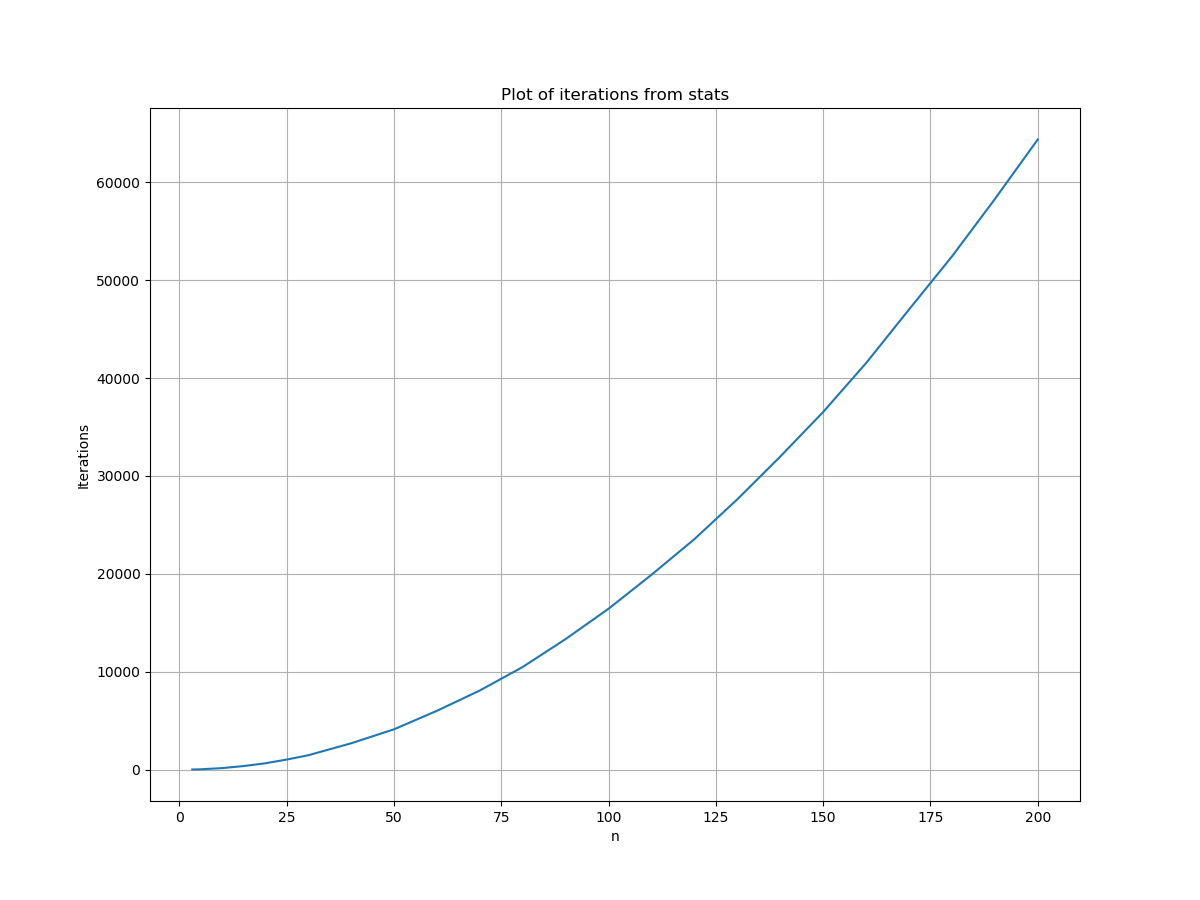
\includegraphics[width = 11cm]{iterations-stats.png}
    %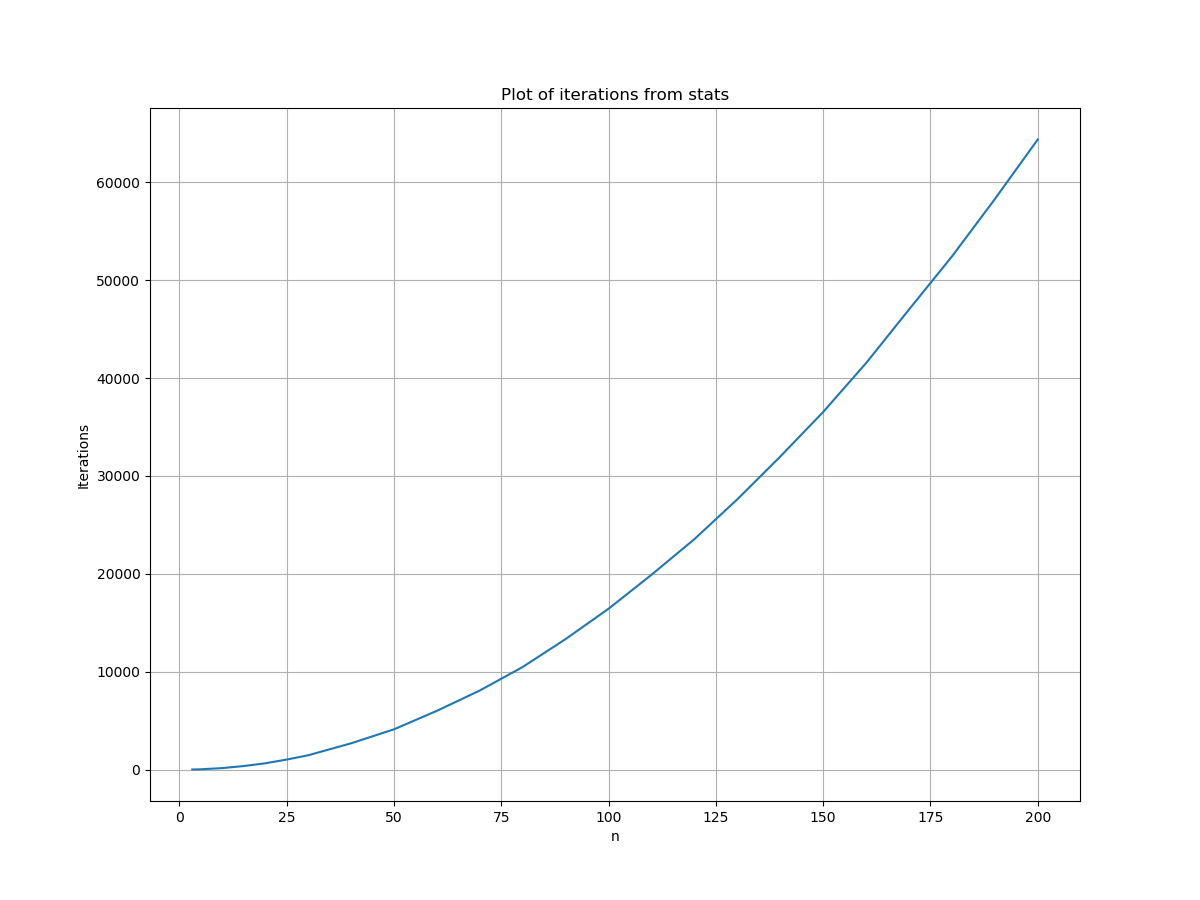
\includegraphics[width = \linewidth]{iterations-stats.png}
  	\caption{The plot of iterations for the Jacobi method as function of the dimension $n$ of the matrix \textbf{A}. }
    \label{fig:iterationspng}
  \end{figure}

  \begin{figure}[ht]
    \centering
    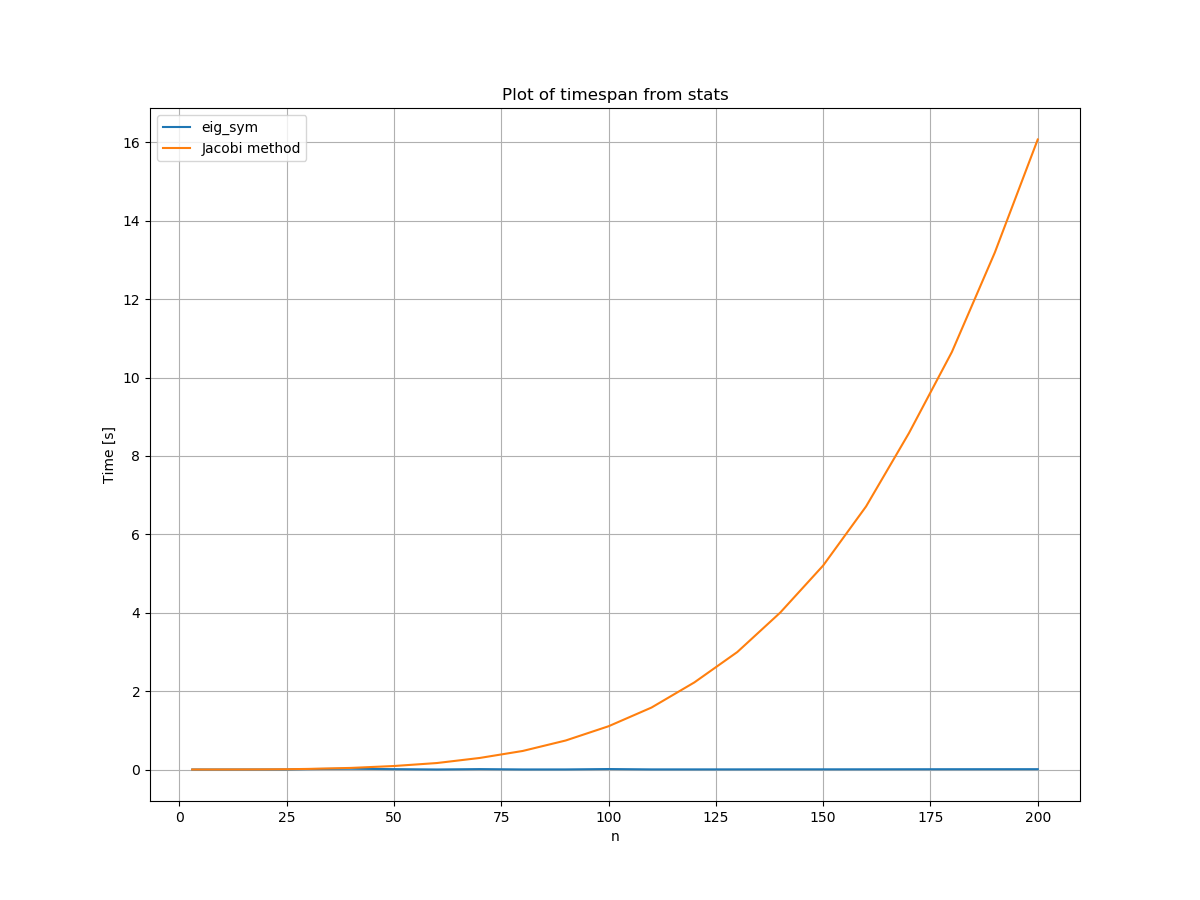
\includegraphics[width = 11cm]{timespan-stats.png}
    %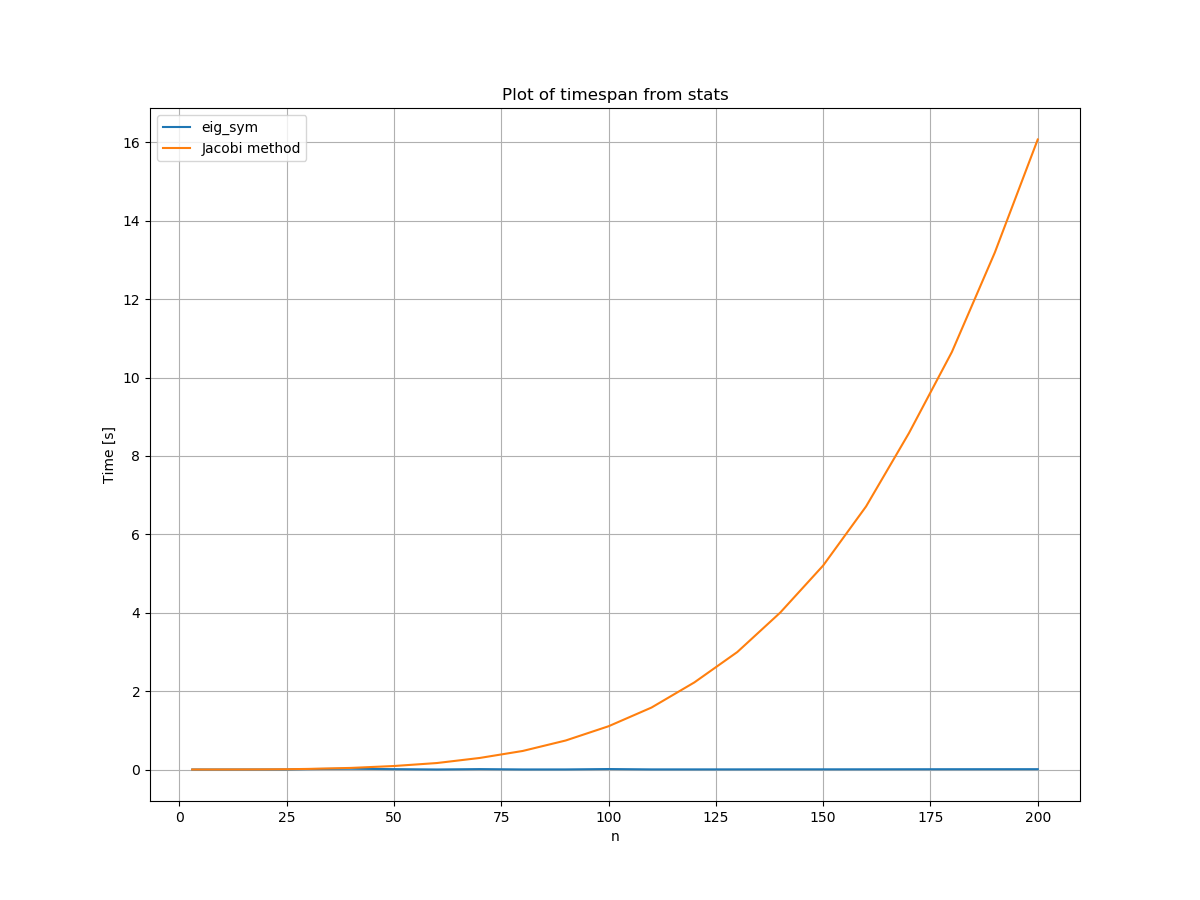
\includegraphics[width = \linewidth]{timespan-stats.png}
    \caption{The plot of the time the function \texttt{eig\_sym} from Armadillo uses and the time Jacobi method uses as functions of the dimension $n$ of the matrix \textbf{A}. }
    \label{fig:timespanpng}
  \end{figure}


\iffalse
  \begin{wrapfigure}{ci}{1.1\linewidth}
    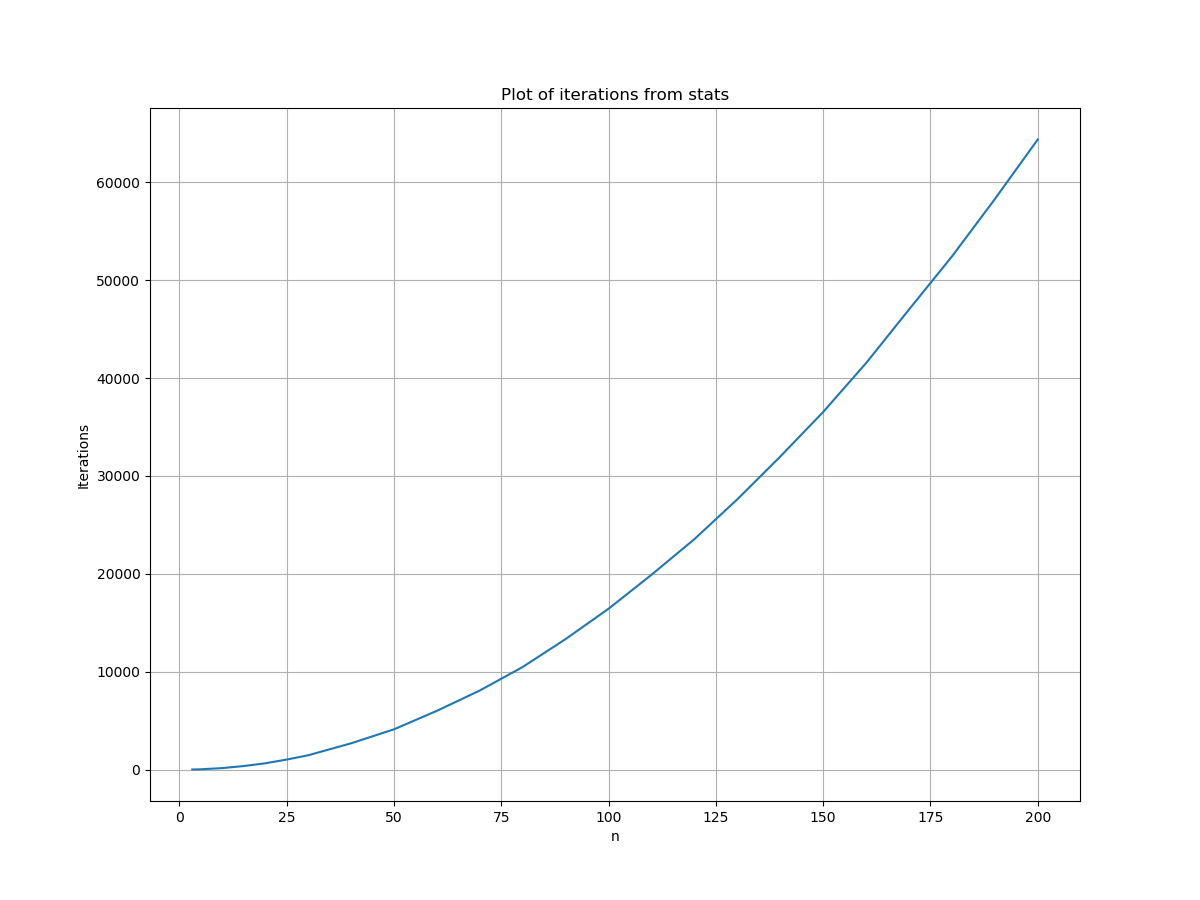
\includegraphics[width=\linewidth]{iterations-stats.png}
    \caption{The plot of iterations for the Jacobi method as function of the dimension $n$ of the matrix \textbf{A}. }
    \label{fig:iterationspngnei}
  \end{wrapfigure}

  \begin{wrapfigure}{li}{1.1\linewidth}
    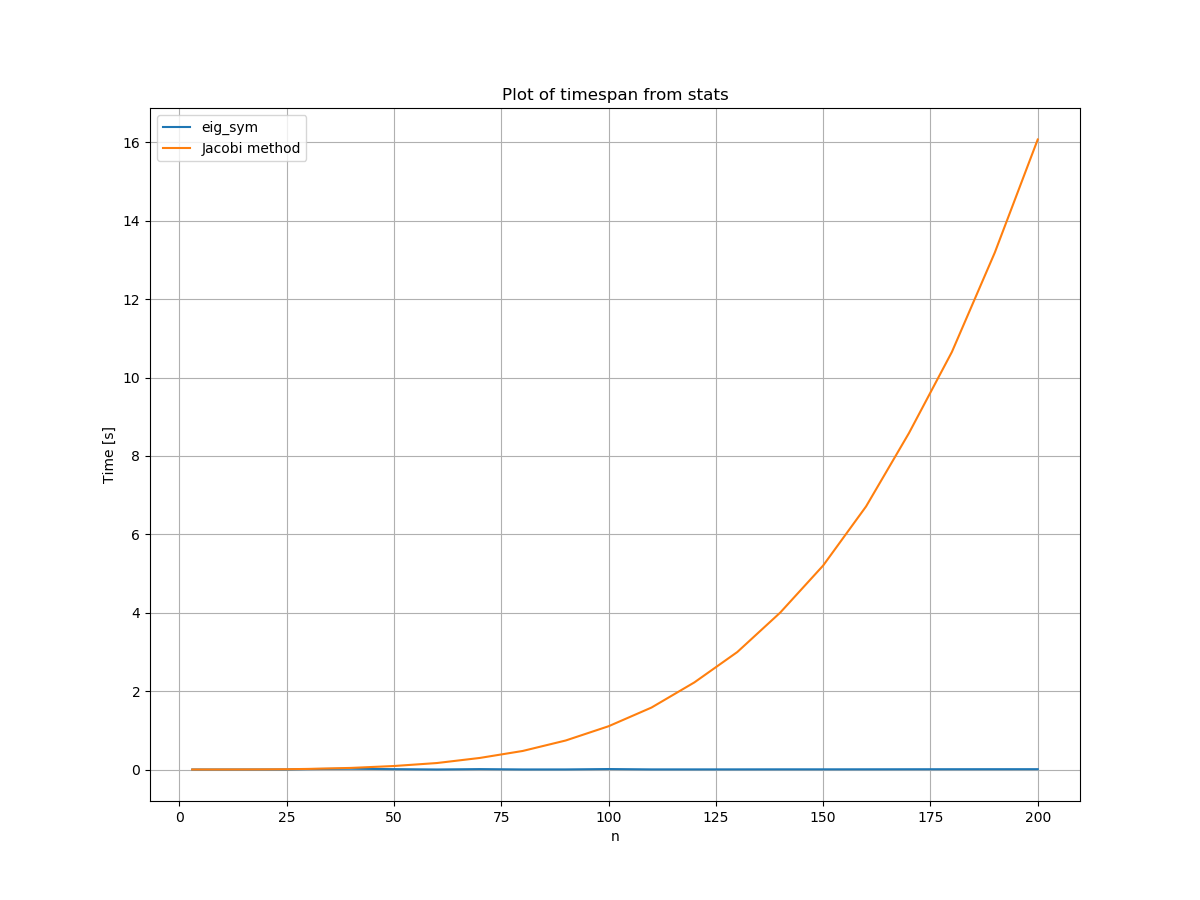
\includegraphics[width=0.5\linewidth]{timespan-stats.png}
    \caption{The plot of the time the function \texttt{eig\_sym} from Armadillo uses and the time Jacobi method uses as functions of the dimension $n$ if the matrix \textbf{A}.}
    \label{fig:timespanpngnei}
  \end{wrapfigure}
\fi

%\clearpage

%\begin{multicols}{2}

  Figure (\ref{fig:iterationspng}) shows that the number of iterations as a function of the dimension $n$ of the matrix has an exponential increase. This means that for larger values of $n$, we need many similarity transformations for our matrix to have all non-diagonal elements become zero. This result coincides with the time difference in the algorithms. We observe that for small matrix-dimensions $n$ our algorithm is sligthly faster than the Armadillo function \texttt{eig\_sym}. When $n$ increases in value, the time used in our algorithm increases exponentially when looking at figure (\ref{fig:timespanpng}). For the biggest given dimension, $n = 200$, our algorithm uses $16$s while \texttt{eig\_sym} uses only $0.008$s. Here we can observe how slow our algorithm is compared to \texttt{eig\_sym}. \\


  \textbf{ferdig med å kommentere dette?}


%\vspace{3cm}


\iffalse
  \begin{table}[ht] \label{tab:exec_time}
    \centering
      \caption{Execution time for the two methods.}
      \vspace{2mm}
      \begin{tabular}{|c|c|c|}
        \hline
        $n$    &   Tridiagonal      &  LU-Decomposition  \\
        \hline \hline
        10   & $2.00\cdot10^{-7}$ & $3.17\cdot10^{-4}$ \\
        100  & $1,40\cdot10^{-6}$ & $1.40\cdot10^{-3}$ \\
        1000 & $1.44\cdot10^{-5}$ & $3.36\cdot10^{-2}$ \\
        \hline
      \end{tabular} \\
      \hspace{0pt}\\
  \end{table}
\fi

%--------------- Discussion ---------------------------------------
\vspace{1cm}

\section{Discussion} \label{sec:Discussion}


  The number of similarity transformations, also called iterations, needed to reach the desired matrix depends on the dimension $n$. For instance a run of our matrix \textbf{A} given as a $(10 \times 10)$ matrix, there are 154 transformations needed. This number is only exact for this specific run, as it will change for any differences to the matrix, both size and elements. \\

  In the lecture notes it states that for the Jacobi method there is no way to predict the number of transformations needed. See this \href{http://compphysics.github.io/ComputationalPhysics/doc/pub/eigvalues/html/eigvalues.html}{file} under \textit{Discussion for Householder's method for eigenvalues}. \textbf{Riktig??} \\

  \textbf{The convergence rate of the Jacobi method is however poor, one needs typically 3n2 - 5n2 rotations and each rotation requires 4n operations, resulting in a total of 12n3 - 20n3 operations in order to zero out non-diagonal matrix elements.} Fra lecture notes. \\




  The Jacobi method is considerably slower for large values of $n$ mainly because the matrix is larger, which means that the algorithm has more elements to rotate and because it has to execute more iterations. The slowness for the Jacobi method is based on when $n$ increases, the algorithm increases the value of some elements, while it decreases the value of others. Consequences of this is that the algorithm has to compute multiple iterations compared to \texttt{eig\_sym} for the same values of $n$.
  Because there is a time difference in the algorithms, we know that \texttt{eig\_sym} does not use the Jacobi method, and is therefore conseiderably faster. The function most likely observes that the matrix is tridiagonal and finds the easiest solution, based on if-else-statements and different types of eigenpair solvers. When looking at the definition of \texttt{eig\_sym} given on this \href{http://arma.sourceforge.net/docs.html#eig_sym}{website}, the function has an argument \texttt{method} for describing two different methods for using the function. The default option is \texttt{dc}, which stands for \textit{divide-and-conquer}, while the other option is \texttt{std}, which stands for \textit{standard}. The \texttt{dc} method is sligthly faster for smaller matrices, dimension $\tilde 300$ and smaller, but for larger matrices it is considerably faster.
  When testing \texttt{eig\_sym} with both methods for matrices of sizes $n = \{ 1000, 5000, 10000\}$ there is already a notable diffrence for $n = 1000$, where \texttt{dc} is ten times faster than \texttt{std}. Because we compute with matrices of dimension $n = 200$ and smaller, the difference in usage of \texttt{eig\_sym} can be ignored as it gives very similar results. \\


    Koden bruker lengre tid både fordi matrisen er større, slik at det er mer å rotere og fordi den må
    utføre flere iterasjoner. \\

    Hvorfor er jacobimethod tregere enn eigsym? økende n, jacobi øker verdien til noen elementer, mens den minker noen andre verdier. altså den fucker noen verdier, mens den fikser noen andre. \\

    eigsym bruker ikke jacobi metoden, og kan dermed være raskere. den kan f.eks. bruke thomas algorithm, som vi programerte i project 1, som er raskere for større matriser. tror den bruker en if-else-statement med ulike algoritmer til å løse de forskjellige matrisene - har prøvd å finne kildefilen gitt ved armadillo, men den finner jeg ikke. \\

    når man skriver inn std istedenfor dc for eigsym er dc litt raskere for store matriser, med n rundt 200, men siden vi driver med relativt små matriser vil man ikke merke stor forskjell. for større matriser, altså 10 i 3 og litt høyere merker man stor forskjell

    eigsym ser at den er tridiagonal og finner letteste løsningsmetode

%---------------Conclusion and perspective---------------------------
\vspace{1cm}

\section{Conclusion and perspective} \label{sec:Conclusion}



%--------------Appendix---------------------------------------------
\vspace{1cm}

\section{Appendix} \label{sec:Appendix}


%----------------------------------------

\subsection{\texttt{jacobimethod.cpp}}

\textbf{Skal kommentere noe for egenverdi og egenvektor?}

Commenting the code \texttt{jacobimethod.cpp}.  OBS. \\

The program starts with defining a function for finding the max values of the off-diagonal elements. This is the function \texttt{offdiag}, which is taken from the lecture notes. The same applies for the function \texttt{Jacobi\_rotate}. \texttt{Jacobi\_rotate} is the function for rotating and computing the matrix. It calculates the equation

\begin{equation*}
    \textbf{B} = \textbf{S}^T A \textbf{S}
\end{equation*}

for finding the diagonal matrix with the eigenvalues of the matrix \textbf{A}. It also computes the eigenvectors, and stores them in a matrix \textbf{R}. \\

In the main function we define the matrix \textbf{A} given by the constants $d$ and $a$. See ? for the definitions of the matrix. Then the clock is set to start, and it times how long the armadillo \\


%------------------------------

\subsection{\texttt{plot\_data.py}}

The program \texttt{plot\_data.py} reads the \texttt{.txt}-file made in \texttt{jacobimethod.cpp} and plots the data. \texttt{jacobimethod.cpp} generates the file \texttt{stats.txt}, which contains the dimension of the matrices, \texttt{n}, the number of iterations, \texttt{i}, the time used for the Armadillo-funtion \texttt{eig\_syl}, \texttt{timespan eig\_sym} and the time used in our algorithm, \texttt{timespan ours}.
\texttt{plot\_data.py} plots the number of iterations needed given by different values of the matrix dimension and it plots the time needed as a function of the matrix dimensions. The values in \texttt{stats.txt} is taken from multiple runs of \texttt{jacobimethod.cpp} for different dimensions of the matrices. The figures (\ref{fig:iterationspng}) and (\ref{fig:timespanpng}) are the plots from \texttt{plot\_data.py}. \textbf{HAR FLERE PLOT Å PLOTTE} \\

\textbf{Skal egentlig kommentere dette?????} \\





%\clearpage

%----------------Refrences----------------------------------------
\vspace{1cm}

\section{References} \label{sec:References}

\href{https://github.com/CompPhysics/ComputationalPhysics/blob/master/doc/Projects/2019/Project2/pdf/Project2.pdf}{Link to the PDF for Project 2}. \\

\href{https://github.com/Erikbgram/Fys3150}{Our GitHub-repository}. \\

\href{https://github.com/CompPhysics/ComputationalPhysics/blob/master/doc/Lectures/lectures2015.pdf}{Link to lecture slides in FYS3150 - Computational Physics}. \\

\href{http://arma.sourceforge.net/docs.html#eig_sym}{Offical Armadillo website for documentation of all contents in the library}. \\

\href{https://journals.aps.org/pra/pdf/10.1103/PhysRevA.48.3561}{Analytical results for specific oscillator frequencies}. \\





%----------------Slutten av dokumentet---------------------------------------



%\end{multicols}

\end{document}
